
\chapter{Cognitive and Affective Probing: A Tutorial and Review of Active Learning for Neuroadaptive Technology}
\chaptermark{Cognitive and Affective Probing}%
\label{chapter:cp}%


{\chaptermeta 

\textbf{Krol, L. R.\textsuperscript{1}, Haselager, P.\textsuperscript{2} \& Zander, T. O.\textsuperscript{3}}

{\small
\textsuperscript{1}Biological Psychology and Neuroergonomics, Technische Universität Berlin, Berlin, Germany
\textsuperscript{2}Donders Institute for Brain, Cognition and Behaviour, Radboud University, Nijmegen, the Netherlands
\textsuperscript{3}Zander Laboratories B.V., Amsterdam, the Netherlands

This is the postprint version of the manuscript published as follows:

Krol, L. R., Haselager, P., \& Zander, T. O. (2020). Cognitive and affective probing: a tutorial and review of active learning for neuroadaptive technology. \emph{Journal of Neural Engineering, 17}(1), 012001. doi:10.1088/1741-2552/ab5bb5\nocite{krol2020cognitiveprobing}
\par}}


\abstract%
\newdimen\origiwspc% slightly adjusting word spacing to better fit the abstract on the page
\origiwspc=\fontdimen2\font%
\fontdimen2\font=0.95\origiwspc%
\emph{Objective:} The interpretation of neurophysiological measurements has a decades-long history, culminating in current real-time brain-computer interfacing (BCI) applications for both patient and healthy populations. Over the course of this history, one focus has been on the investigation of cortical responses to specific stimuli. Such responses can be informative with respect to the human user's mental state at the time of presentation. An ability to decode neurophysiological responses to stimuli in real time becomes particularly powerful when combined with a simultaneous ability to autonomously produce such stimuli. This allows a computer to gather stimulus-response samples and iteratively produce new stimuli based on the information gathered from previous samples, thus acquiring more, and more specific, information. This information can even be obtained without the explicit, voluntary involvement of the user.
\emph{Approach:} We define cognitive and affective probing, referring to an application of active learning where repeated sampling is done by eliciting implicit brain responses. In this tutorial, we provide a definition of this method that unifies different past and current implementations based on common aspects. We then discuss a number of aspects that differentiate various possible implementations of cognitive probing.
\emph{Main results:} We argue that a key element is the user model, which serves as both information storage and basis for subsequent probes. Cognitive probing can be used to continuously and autonomously update this model, refining the probes, and obtaining increasingly detailed or accurate information from the resulting brain activity. In contrast to a number of potential advantages of the method, cognitive probing may also pose a threat to informed consent, our privacy of thought, and our ability to assign responsibility to actions mediated by the system. \emph{Significance:} This tutorial provides guidelines to both implement, and critically discuss potential ethical implications of, novel cognitive probing applications and research endeavours.
\fontdimen2\font=\origiwspc%


\clearpage


\fancypagestyle{cp}{%
    \fancyhf{}
    \fancyhead[EC]{\textit{\leftmark}}
    \fancyhead[OC]{\textit{\rightmark}}
    \fancyfoot[C]{\thepage \\ \vspace{9.9mm} \colorbox{footerbg}{\parbox{\paperwidth-2\fboxsep}{\centering\parbox{0.75\paperwidth}{\centering\fontsize{9pt}{9pt}\selectfont\textcolor{footerfg}{This is the postprint version of published manuscript: Krol, L. R., Haselager, P., \& Zander, T. O. (2020). Cognitive and affective probing: a tutorial and review of active learning for neuroadaptive technology. \textit{Journal of Neural Engineering, 17}(1), 012001.}}}}}
    \fancyfootoffset[]{1.25in}}
\pagestyle{cp}


\section{Introduction}

One essential skill required of disc jockeys (DJs) is the ability to ``read the crowd''. In order to maximise the audience's enjoyment, a DJ may play different songs and gauge the reaction they evoke \cite{gates2006dj}. Depending on this reaction, the DJ decides whether or not to end the current song early, and what to play next. This is an iterative process that continues to optimise with each played song, the goal being maximum audience participation, or indeed, maximum audience happiness.

The feedback from the audience is essential input in this process. However, the audience members themselves are not necessarily aware of providing any---their responses are mostly automatic, even reflexive. Hardly would one deliberate whether or not the current chords are sufficiently engaging; rather, the rhythm and mood of the music will simply induce the audience members to express themselves in a certain way, and it is this expression that the DJ will read and use as input.

In this tutorial, we will discuss a situation analogous to the one above, in the context of human-computer interaction (HCI): An adaptive process where a computer presents something that automatically evokes a response from the user, which the computer can then interpret and use for further processing. We will discuss the methods involved, how they relate to past and current applications, and what aspects must be considered going forward with this technology.

Let us first discuss what an ``automatic'' response may be in the context of HCI. In traditional HCI, all input that we give to the computer is based on goal-oriented, explicit, voluntary actions. By \emph{explicit communication}, we mean any intentional action performed for the purpose of communicating specific content. For example, to communicate information to a computer, we must actively type, say, click, move, swipe, or select things in a corresponding fashion, or nothing will happen. 

There are technologies that give a computer access to more information about the user than what is explicitly communicated. In virtual reality, moving our arms and legs provides explicit positional information to the computer, but, going beyond that, full-body motion tracking can also be used to analyse these movements, or the resulting postures, for additional information that was not meant to be communicated \cite{kleinsmith2011posture}. Your movements may reveal that you are happy or sad, or perhaps drunk. Similarly, for example, facial recognition can be used to assess emotions \cite{janssen2013emotionrecognition}, and passive brain-computer interfaces can analyse our brain activity in order to supply implicit input to a computer \cite{zander2011,krol2018interactivity}. By \emph{implicit communication}, we mean that information is acquired from output that was not intended to communicate that information. Here, we focus on methods that target our brains---the primary seat of cognition and conscious experience---as they are uniquely positioned to infer information about us in such a way.

Real-time detection of mental states has been demonstrated as early as the 1970s \cite{vidal1977}, and since then, further research has shown that BCI methodology can be used to detect a range of different patterns of brain activity, including some that reflect specific cognitive and affective processes \cite<e.g.,>{donchin1981,hillyard1998visualselectiveattention,yeung2004reward}. These mental processes occur naturally during our everyday lives. So-called \emph{passive} BCI systems \cite{zander2011,krol2018interactivity} target such naturally-occurring mental states in order to provide \emph{implicit input} to a computer \cite{schmidt2000,zander2014implicit}. In other words, passive BCI systems rely on brain activity that was not \emph{intended} by the user to provide information to those systems, but is nonetheless used as such. 

It should be noted, however, that our current ability to discern different mental states, and thus our ability to infer specific information from brain activity, is limited. While research into ``reading'' mental states in novel ways continues to move forward \cite<e.g.,>{haynes2011brainreading,huth2016semanticmaps,senden2019mentalimagery}, it is not currently possible to infer the propositional content of thought \cite{haselager2018reading}. 
Thus, in many cases, additional information about the current situation is required in order to draw meaningful inferences from measured brain activity \cite{makeig2009mobi,zander2012context}. 
For example, when high workload is detected in a multi-tasking environment, additional information is required to make an optimal decision on which task to automate \cite{muhl2014crosscontextworkload,krol2016workload}. Similarly, when error processing is detected, it is important to know where that error originated \cite{falkenstein2000,mousavi2019error,wirth2019errorcategorisation}. 
Determining the best way for a computer to sense, filter, and represent relevant situational aspects remains an open field of research with many different approaches \cite{perera2014contextsurvey}. 

In our earlier analogy, if an observer to the DJ's performance sees the crowd's reaction but cannot hear and does not know what music is currently playing, they will be none the wiser, until they obtain this extra piece of information. The DJ, on the other hand, doesn't only know what music is playing---she is the one who selected the music in the first place!

Similar to a DJ, in HCI contexts where a computer has control over relevant situational aspects as well as access to mental state measurements, it can also \emph{actively induce an event in order to assess the user's brain response to it}. This allows it to \emph{probe} the human user. Having a computer induce an event itself circumvents the need for elaborate post-hoc context sensing. Rather than waiting for events to occur naturally in order to learn the relation between events and mental states, the computer can purposefully generate specific events and gauge the user's implicit response. Doing this in an iterative fashion allows the computer to adaptively pursue a particular goal. As we will see, these events can also be ``hidden'', embedded in the ongoing interaction itself. Furthermore, considering that humans are generally unable to stop their brains from automatically processing perceived stimuli, the computer is effectively posing a question directly to the user's brain, potentially bypassing the user's explicit faculties.

In essence, this \emph{cognitive probing} can be seen as a form of \emph{active learning} \cite{settles2009activelearning}. Active learning is a concept in machine learning where a learner, rather than simply accepting samples as they come, has control over which samples it learns from. Cognitive probing applies this concept to a computer learning from implicit responses to technological state changes, with the added notion that the learner in this case is not merely responsible for its own learning, but also for the effect its sampling has on the human. Inducing mental states is not a neutral act.

Learning itself can be the sole goal of the computer. However, additional goals may be pursued as well: much like the DJ's goal of maximum audience happiness, the computer, too, may attempt to find stimuli that maximise certain psychological states. As such, cognitive probing can be a powerful tool to realise closed-loop neuroadaptive technology. Neuroadaptive technology is technology that adapts itself based on implicit input of neurophysiological origin (Zander \& Krol et al., 2016). The amount of input obtained by such technology, and the efficiency with which it is obtained, can be greatly increased using cognitive probing. In particular, the technology can iteratively adapt itself to the user based on implicit information gathered from probe-induced brain activity. 

The use of passive BCIs for cognitive probing thus provides a potentially powerful method for a computer to unobtrusively obtain information about its users. At the same time, it also represents a potentially dangerous and psychologically invasive method concerning mental privacy, and hence its application must be handled with due care and transparency \cite{mecacci2019criteria}.

In this tutorial, we first introduce and explain a general, broad definition of this method. We provide examples from the literature, pointing out that cognitive probing, as defined here, has already been used for at least three decades in different ways and different fields. With recent advances in neurophysiological sensing \cite{mullen2015dry,zander2017dry} and neuroadaptive technology (Zander \& Krol et al., 2016; \citeNP{lorenz2017neuroadaptivebayesian}), however, we believe it is prudent to now unify these methods previously considered disparate in a single framework, and to present a careful consideration of the different aspects involved. Therefore, a further section discusses a list of aspects, characteristics, and other considerations that are relevant to the use of cognitive probing in different applications, and to society at large. We conclude with a speculative vision of the future, highlighting possible research endeavours.


\section{Cognitive Probing}
\label{sec:definition}

At the basis of our proposed definition lies a single probe, where: \newline

\textbf{A cognitive (or affective) probe is a technological state change that is initiated or manipulated by the same technology that uses it to learn from the user's implicit, situational, cognitive or affective brain response to it.} \newline

\emph{Cognitive probing} or \emph{affective probing}, then, is the repeated use of probes in order to generate a model in which the learned information is registered.\footnote{The definitions given here for cognitive probe and cognitive probing supersede the earlier working definitions presented in \citeA{krol2018cp}.}

We use cognitive probing as the general term including both cognitive and affective probing; the term affective probing can be used in cases focusing exclusively on affect \cite{zander2009affective}. Also note that the base definition refers to a single probe, i.e. a single state change eliciting a single response. Technically, meaningful learning can be done using a single probe: given sufficiently accurate tools, a single probe may be sufficient to provide adequate information. However, the main potential, and main focus, of the method lies in the adaptive, sequential use of multiple probes.

We will now discuss the definition's constituent elements in more detail.

\paragraph{Technological state change.} A technological state change is any action undertaken by a piece of technology. We use the term \emph{technology} to collectively refer to any and all (connected) technological elements in any potential situation. With a technology's \emph{state} being its specific current configuration, a \emph{technological state change} is thus any change in configuration that the technology undergoes. 

In neurophysiological experiments, the presentation of cues, stimuli, or feedback would be an example of a state change. In the example of an automated, neuroadaptive DJ, it could be a song that is started.

\paragraph{Initiated or manipulated.} Most technological state changes that a user will notice are user-generated, i.e. commanded by the user themselves, with the technology reacting to explicit input. Non-user-generated events include e.g. notifications of incoming e-mails or low battery. A cognitive probe refers to a state change whose occurrence, form, or timing was at least partially produced by the technology itself, and not by the user. This thus requires that the technology has some degree of control over its own state changes.

Technology can initiate a state change for the sole or primary purpose of obtaining a response, i.e. to produce a probe for the probe's sake. When a potentially informative state change occurs for other purposes, user-generated or otherwise, the system can manipulate it so as to serve as a probe, for example by adjusting its form or timing.

In the example started above, it is important that the neuroadaptive technology itself somehow influences the song, as opposed to a human user simply pressing ``play''. The manipulation can take different forms: among other options, it could be that the user requests music to be played in general, upon which the technology selects the song; it could be that the music has been pre-selected but the technology decides when to play it; or it could be a process chain initiated entirely by the technology itself. In any case, the technology does initiate or manipulate the technological state in question, as opposed to this being decided entirely by the human.

\paragraph{The user's implicit, situational, cognitive or affective brain response.} Cognitive probing focuses on \emph{brain responses}: brain activity (or a change in brain activity) that is elicited as a function of specific events. To be a cognitive probe, a technological state change must thus in one way or another elicit brain activity, or a change in ongoing brain activity, which can in turn be detected by the technology.

``Cognitive or affective'' is spelled out here to distinguish it from more elementary brain activity such as the auditory brainstem response or steady-state visually evoked potentials. Since these responses do not inherently reflect cognitive or affective processing, they cannot be used for cognitive probing.

Furthermore, we limit this definition to information taken from the brain response that was not intended to be communicated to the technology---cognitive probing targets \emph{implicit} human-computer communication. 

``Situational'' means the implicit brain response is automatically registered alongside parameters of the current situation. An ability to interpret ongoing brain activity taken in and of itself results merely in a stream of mental state assessments. In order to learn something from these mental states, they must be combined with additional information about the situation in which these mental states occurred. Cognitive probes ensure that at least one piece of situational information is available: the probe itself. 

Further situational aspects can of course be included, dependent on the accuracy with which they can be sensed and/or represented \cite{perera2014contextsurvey}.

By co-registering the interpreted brain responses with all related situational information, a \emph{user model} is formed. Over time, such a model will come to reflect regularities in the users' responses and thus allow aspects of higher cognition functions to be inferred, as e.g. in Zander \& Krol et al. (2016).

Continuing our example, the music that starts playing will evoke a response from the human listener---for example, they may like or dislike the song, it may distract them or evoke a pleasant memory. The listener does not intentionally produce this response; it is simply a result of them being human, and hearing the song. The response is reflected in their brain activity.

\paragraph{The same technology that uses it to learn.} The brain response induced by the probe is detected and registered in a user model alongside additional available information. The purpose of this is to learn: each response is decoded to provide at least one bit of information in order to reduce previous uncertainty or to adjust existing knowledge. This knowledge is represented in the model.

Importantly, the learner is the same technological entity that produced the probe. Combining the technological ability to interpret ongoing brain activity with the ability of that same technology to actively elicit this brain activity is what allows probes to be purposefully generated to fulfil a specific goal. An independent, external event, even if the technology interprets it and learns from it as described above, is not a cognitive probe because the technology had no influence over it. 

Finishing the example, the automated, neuroadaptive DJ measures and interprets the listener's implicit brain response to the song, and learns that they do or do not like this music. It uses this information to select the next song accordingly.

\begin{figure}[t]
    \centering
    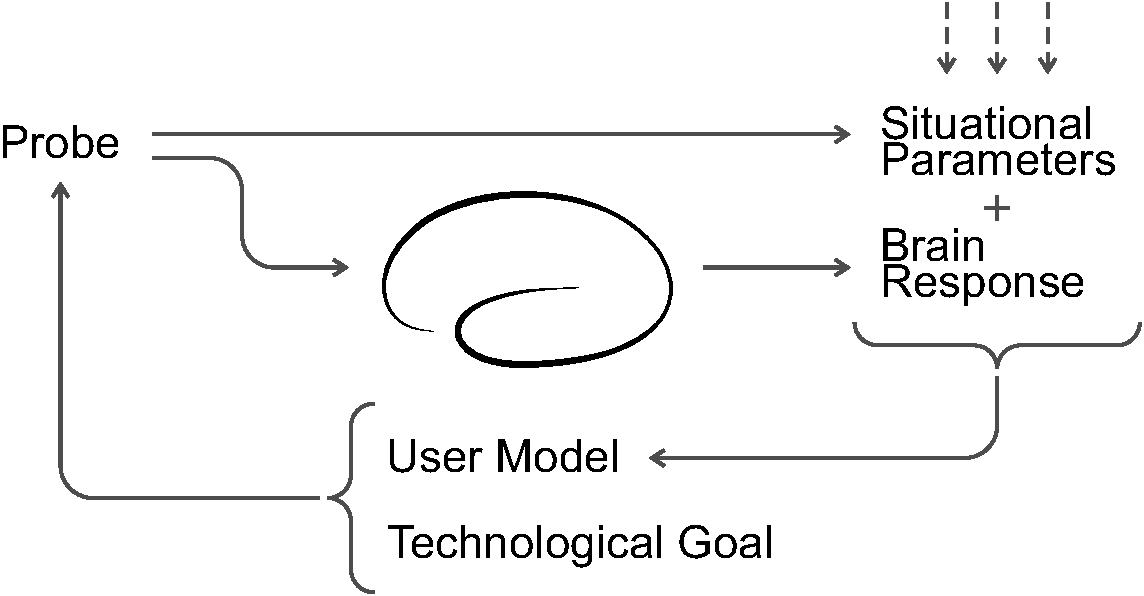
\includegraphics[width=10cm]{figures/cp-diagram.pdf}
    \caption[Diagrammatic overview of the cognitive probing mechanism.]{A diagrammatic overview of the cognitive probing mechanism. Based on available information, the technology initiates or manipulates a state change---a probe. This change elicits a brain response. Together with parameters describing the probe as well as, optionally, additional parameters describing the situation in which the user's response happened, the technology interprets this response and updates the model, increasing the accuracy of the information available to it for the next goal-oriented probe. At a minimum, the situation is described by the probe itself, but any other relevant parameters can be included.}
    \label{fig:cp:diagram}
\end{figure}

\paragraph{Summary.}
Figure~\ref{fig:cp:diagram} shows a diagrammatic overview of the cognitive probing mechanism. A probe elicits a certain response in the user's brain. The neuroadaptive technology measures this response, along with relevant parameters of the state change, and co-registers these pieces of information alongside one another in a user model. The combination of all pieces of information in the model allows inferences to be drawn. Based on the user model and the current goal of the technology, the next probe is initiated. This again elicits a response, leading to an update of the user model. 

To further delineate the method of cognitive probing, we mention a number of counter-examples in the discussion section of applications that are closely related to cognitive probing, but fall outside of this definition. For now, we will first turn to a number of past and present applications and experiments that do fit this definition, to illustrate the method.


\section{Literature Review}
\label{sec:literature}

The proposed definition of cognitive and affective probing is deliberately generic, and does not specify, for example, for what purpose the learned information is to be used, or how inferences are to be made. Therefore, we can identify a number of past and present methods that fit this definition. Although these methods have been treated disparately before, we can see that the same terminology applies.

We may say that the history of cognitive probing starts with the \emph{event-related potential} (ERP) technique \cite{luck2014erp}. This was the first of a number of techniques that allowed researchers to associate the brain's neuroelectric responses with specific events. Initially, the ERP technique was used both to elucidate the neural pathways involved in sensory processing \cite<e.g.,>{cobb1960erp}, and as a diagnostic tool to assess the (mal)functioning of the involved structures and processes \cite<e.g.,>{chiappa1997clinicalep}. Later, it was demonstrated that ERPs also reflect aspects of cognitive processing \cite{walter1964cnv}.

The ERP technique has been used in various applications and research endeavours. For example, \citeA{fischer1999mmncoma} used a mismatch negativity paradigm \cite{naatanen2007} to assess levels of consciousness in comatose patients, by presenting them with sentences that did or did not make semantic sense. \citeA{farwell1991gkt}, based on earlier work by \citeA{rosenfeld1988erpgkt}, presented participants with pictures of objects that did or did not belong to a crime scene in order to infer whether or not they had incriminating knowledge of it. 
Most ERP studies, however, including these two examples, do not employ automatic learning by the same computer that produces the stimuli, meaning they do not employ cognitive probing as such. Instead, the average ERPs are examined post hoc by the researchers. A key element that was missing was the ability to detect and analyse brain responses in real time. This had been demonstrated first in the 1970s \cite{vidal1977}, but resurfaced more prominently in the 2000s with the advent of machine learning in EEG research \cite{ramoser2000,blankertz2002singletrial,lotte2007classificationreview}. 

This development is clearly seen in reactive BCI applications \cite{zander2011}, where ERPs are elicited and used to assess correlates of human attention to allow users to voluntarily control applications. In particular, mental spellers highlight or present different letters of the alphabet on a display, in order to learn which letter was attended to \cite{farwell1988,treder2011gazeindepbci}. Each such presentation results in an ERP. Because ERP responses to attended letters are known to be different from those to unattended ones, the system can detect this in real time and learn which letter the user intended to write. These highlights and presentations are examples of cognitive probes: they are solely initiated for the purpose of learning which letter the user wishes to communicate. Later developments added adaptive probing techniques where the sequence of highlights was adapted in real time to the available information \cite<e.g.,>{lenhard2008adaptivep300,jin2011p300flashpattern}, or where intermediate feedback elicited additional brain responses \cite{dalseno2010}. Finally, \citeA{mladenovic2019activeinference} present an elaborate implementation of a mental speller that combines multiple adaptive strategies using a single framework based on active inference. Here, a prominent user model is used to generate the system's actions, the user's brain responses to which in turn are used to update that user model. This is a clear example of cognitive probing in the current sense of the term.

A similar development from independent analyses of brain activity to cognitive probing as described here happened in the field of neuroergonomics  \cite{parasuraman2003neuroergonomics}, where ERPs have been used for, among other things, workload detection. It has long been shown that certain features of brain responses to rare sound events seemingly reflect the availability of attentional resources \cite{sirevaag1989p300resource}. This led to the development of the secondary oddball task, where sounds are played repeatedly and intermixed with rare deviant sounds. Real-time evaluation of the brain responses to these tones then allow real-time inferences to be made with respect to available resources, i.e., workload. In such a context, the tones are thus cognitive probes, allowing the same technology that produces them to learn about the cognitive state of the user. This has been used in online, closed-loop contexts, where e.g. additional tasks are automated or postponed when high workload is detected in order to alleviate the load \cite{kohlmorgen2007}. Secondary oddball tasks have also been shown to work in demanding real-world scenarios \cite{dehais2018monitoringfatigue}.

In the previous examples, the state changes making up the probes were induced for the sole purpose of learning. However, this must not necessarily be the case: probes can also be embedded in state changes that are produced for other reasons. One example of this is the presentation of feedback in such a way as to elicit an error-related potential when the presented information is false or undesired \cite<e.g.>{dalseno2010}. Presentation of feedback is obviously an inherent part of any interactive system, its primary purpose being to 
inform the user. Its presentation can, however, be controlled by the computer allowing it to be used as a cognitive probe.

Similarly, \citeA{kirchner2016multirobotcontrol} effectively embedded a type of secondary oddball task in an otherwise natural human-computer interaction. During a multi-robot control task, participants had to pay attention to task-relevant messages that were presented during the interaction. The appearance of these messages evoked brain responses with properties comparable to those evoked by a dedicated secondary oddball paradigm. This allowed the computer to deduce an index of task engagement from these responses, and adapt the presentation of the messages-cum-probes accordingly. This shows that probes can be effectively hidden in natural aspects of an already-ongoing interaction.

It is even possible to have probes be the primary basis of the interaction. \citeA{zander2014implicit,zander2016nat} as well as \citeA{iturrate2015teaching} demonstrated applications where this was the case: the guidance of a cursor or a robotic arm, respectively. Each movement of the cursor or arm elicited an ERP that could be automatically interpreted as reflecting the appropriateness of that movement with respect to reaching a target position. The initial movements occurred randomly. Based on the information gathered from the observer's brain response following each movement, however, a dynamic user model could be generated reflecting which behaviours were perceived positively, and which were perceived negatively. Based on this model, the movements could be steered into the apparently desired direction, towards the target. While \citeA{iturrate2015teaching} suggest this to be used for voluntary prosthetic control, Zander \& Krol et al. (2016) stress that the elicited responses themselves appear to be involuntary. In fact, their participants were unaware of having any influence over the cursor. As such, this method allowed the cursor to be controlled entirely implicitly.

This latter example presents a sliding scale with respect to the primary purpose of each cursor movement. In a process later also described by \citeA{hincks2017entropicbci}, the stimuli were initially selected at random, with no other purpose than to populate the user model. As information was gathered and a user model was formed, the stimuli became increasingly part of the task completion (target reaching) mechanism while still allowing for new information to be learned.

A similar concept has been developed in the context of neuroscientific experimentation. Whereas traditional experiments are generally informed by specific hypotheses and employ correspondingly narrow experimental designs, a neuroadaptive approach to hypothesis testing would allow an experimental computer to present different stimuli or conditions in search for a specific neurophysiological response pattern \cite{lorenz2017neuroadaptivebayesian}. For example, in order to find which stimuli optimally activated select cortical regions, \citeA{lorenz2016automaticneuroscientist} used functional magnetic resonance imaging (fMRI) to assess the participants' responses to a range of audiovisual stimuli reflecting different physical properties. Rather than presenting all stimuli in order to analyse the different responses post hoc, responses were assessed in real time. Subsequent stimuli were automatically selected based on previously gathered responses, with the aim to learn the parameters that elicit a maximum response. This closed-loop, neuroadaptive experimental design thus employs cognitive probes in order to learn how the participant responds to certain stimuli. Once the optimal stimuli have been found, the experiment can continue to gather data for further investigation.

A final example concerns the generation of a dynamic user model reflecting user interests \cite{wenzel2017wordrelevance}. Here, the brain responses were not elicited by the presentation of the stimuli directly, but by the participant's eye fixation on them: the stimuli were already visible, the participants' gaze was tracked, and brain activity was analysed relative to the eyes fixating on each stimulus using so-called fixation-related potentials (FRPs; \citeNP{dimigen2011frp}). The stimuli were words of different semantic categories. By combining fixation information and an interpretation of the FRPs, the authors were able to assess which words were relevant and which were not, and ultimately, to infer which category of words the participant was interested in. This illustrates that the brain response to a specific probe (presenting the words) need not be immediate, but can be delayed. In this case, it was delayed until the participant fixated on it. This also illustrates the potential relevance of additional context information. \citeauthor{wenzel2017wordrelevance} combined the brain response with information about the participant's gaze in order to infer the semantic category of current interest.

Aside from fMRI and the EEG-based ERP technique, which featured heavily in this section, frequency-based measures can of course also be used \cite<e.g.,>{ewing2016tetris,mousavi2017mi}, as well as other modalities, such as functional near-infrared spectroscopy (fNIRS) \cite<e.g.,>{afergan2014dynamicdifficulty,yuksel2016bach}. 

In these examples from different areas of research, we see a convergence towards the idea of using real-time, single-trial analyses in an automated, closed-loop fashion in order to learn something about the human user or participant---i.e., towards the idea of cognitive probing presented here. While clearly sharing common methodologies, the used terminology is still disparate: authors referred to their methods, or parts thereof, as ``probing'' (\citeNP{kane2000erpcoma}; Zander \& Krol et al., 2016), ``brain reading'' or ``embedded brain reading'' \cite{kirchner2019embeddedmmi}, ``exploration'' \cite{iturrate2015teaching}, ``active sampling'' \cite{lorenz2017neuroadaptivebayesian}, ``active inference'' \cite{mladenovic2019activeinference}, or implied the method to be part of an ``entropic BCI'' \cite{hincks2017entropicbci}, of ``adaptive'' systems \cite{schultheis2004textdifficulty,yuksel2016bach}, or of a system using ``brainput'' \cite{solovey2012brainput}. This is part of the reason why we now present a unified framework and terminology.

In the next section, we discuss a number of aspects of cognitive probing that determine how implementations may differ, and aspects that are important to consider when developing systems that employ this method. In some cases, these overlap with general active learning aspects and guidelines; in others, cognitive probing must be treated separately due to its utilisation of brain data gathered directly from human beings.


\section{Aspects and Considerations}
\label{sec:aspects}

Cognitive probing can be applied in different ways and across different contexts, to suit different purposes. This section lists a number of ways in which these differences can be realised. This serves both to illustrate concepts, techniques, and possibilities of the cognitive probing method, and as a list of considerations and trade-offs for researchers and developers.

Furthermore, the cognitive probing method raises a variety of ethical issues that we will briefly introduce and discuss in this section. The basic concern centres around the implications of probing someone's brain processes in order to gather cognitive or affective information about that person. A responsible use of such technology requires, at the very least, reflections on the topics of privacy and consent, and responsibility for actions mediated by the technology. 


\subsection{Learning Strategies}
\label{sec:strategy}

Probes are designed in order to obtain information. Two central questions are thus: What information is to be obtained, and how is this best achieved?

Ultimately, the information that can be obtained of course depends on the cognitive and affective states that can be detected and the reliability of these assessments. Here, traditional neuroscientific considerations apply. See e.g. \citeA{brouwer2015pitfalls} and \citeA{gerjets2014workload} for recommendations.

There are different possible strategies to learn from cumulative samples and to choose subsequent probes. In the previous section, \citeA{lorenz2016automaticneuroscientist} and \citeA{mladenovic2019activeinference}
used Bayesian inference and optimisation \cite{snoek2012bayesianoptimization}, whereas \citeA{iturrate2015teaching} used a form of reinforcement learning \cite{sutton1998reinforcementlearning}. 

With its abstract similarity to active learning, the cognitive probing method can utilise many of the so-called query strategies of active learning \cite{settles2009activelearning}. As illustrated in Figure~\ref{fig:cp:diagram}, the system can select a specific state change based on the knowledge currently available in its model, in order to update that model (i.e., to fulfil its goal of learning). It can thus use available information in order to determine which change will be initiated, and to what end.

One strategy to that effect that \citeA{settles2009activelearning} mentions is \emph{uncertainty sampling}: the system can initiate changes along those dimensions about which it has the least knowledge. For example, if the system has no information pertaining to a particular condition, it could deliberately produce this condition in order to probe the user's response to it. 

Other strategies can similarly be applied, notably \emph{expected model change} (obtaining information that would most change the model) and \emph{expected error reduction} (to reduce the error in the model, or in the system's behaviour). A system may initialise using random variables and based on these initial samples, move to specific strategies to find more suitable values \cite{hincks2017entropicbci}.


\subsection{Repeating Probes}

Most likely, it will be necessary to probe multiple times in order to draw reliable conclusions. Given imperfect measurement or inference methods, a trade-off needs to be considered between the number of probes and the accuracy of the gathered information.

With respect to obtaining a specific piece of information, a sequence of probes can be presented in different ways. One way is to present a precisely defined state change a pre-determined number of times (e.g., once, or ten times). The optimal number of repetitions has, for example, been investigated for P300 spellers \cite<e.g.,>{jin2011p300flashpattern}. Another method is to use a confidence criterion, where the state change is repeated until a certain level of confidence has been reached (i.e., the error reduction strategy combined with dynamic stopping; \citeNP<e.g.,>{schreuder2013dynamicstopping}). Finally, rather than repeating the same probe, the probe itself could be dynamically changed during the sequence, adaptively homing in on increasingly specific information of interest as e.g. in \citeA{lorenz2017neuroadaptivebayesian}. 


\subsection{The Roles of Time}

Time is relevant in a number of ways. For one, time itself may be one of the relevant situational factors to be included in a model: the absolute time of day (e.g., to learn patterns that are different in the evening as compared to the morning), or the time relative to a previous event.

Also the time needed for the system to measure and process the brain response can have practical importance. Sometimes the measurement and data analysis might take longer than what is useful for a particularly time-critical application.

Furthermore, the duration of a probe's effect needs to be considered. In the examples given in this paper so far, all relevant brain responses to the probe were near-immediate. However, this need not always be the case. Depending on the application, a distinction can be made between up to four time points or periods: the time that the probe is generated (i.e., the technological state is changed); the time that the probe is perceived; the period of time during which the probe's influence remains apparent (i.e., during which relevant brain responses can be gathered); and the period of time during which the gathered information remains valid.

The first two time points are usually the same, but not necessarily. It is possible for a probe to be noticed only after it has been produced, as for example in the fixation-related study mentioned above \cite{wenzel2017wordrelevance}. It may also be possible for a state change not to be consciously noticed at all, while still having an effect \cite{negri2014subliminal}. The third point covers a time period that varies depending on factors such as habituation, and the time it takes for a meaningful response to arise---see also section~\ref{sec:impulsive} for the difference between impulsive and reflective responses. The final point concerns the ``half-life'', so to say, of any gathered information. Is it generally valid and can it remain in the model indefinitely, or may the user's responses change over time such that the learned information becomes obsolete? In the latter case, the probes may need to be repeated at certain intervals.


\subsection{A Probe's Purpose}
\label{sec:purpose}

The presented definition requires that probing must be done in order to learn. This does not mean, however, that learning is necessarily the only objective: the system may simultaneously have other goals.

Figure~\ref{fig:cp:diagram} illustrates three effects of a probe: its effect on the environment (at a minimum, this is simply the occurrence of the probe itself), its effect on the brain (the brain response elicited by the probe), and ultimately, the adjustment of the model. The goal of ``learning'' refers to this last effect. However, cognitive probes can be selected to simultaneously fulfil further strategic goals. In particular the second consequence, the user's response, can be part of the goal-driven behavioural strategy of the system.

The system may aim to induce or sustain desirable psychophysiological user states. If certain probes have been learned to lead to positive responses, the system may aim to induce or sustain the user's positive state by repeating such probes. This was the case for the implicit cursor control experiment (Zander \& Krol et al., 2016): each probe served both to further the system's knowledge of the preferred direction, and to steer the cursor into that direction.

Note that goals need not remain static over time: for example, an initial phase of mere information-gathering can be followed by different goals as decided based on the gathered information, or goals may change based on changing situational aspects.

Furthermore, even when learning is the main objective to employ cognitive probing itself, the purpose for which information needs to be learned is left entirely open.

In other words, it can be said that neuroadaptive systems have their own agenda \cite{fairclough2017intadapt}. An important factor to consider is whether or not, or to what extent, this agenda is in line with the user's own goals, discussed in more detail further below.


\subsection{Interference and Distraction}
\label{sec:interference}

The fact that cognitive probes are intended to elicit a response means that they must influence the user in one way or another. As mentioned above, this influence can be used by the system for a higher goal, such as the promotion of a desired mental state. At other times, this influence may be an unwanted side-effect. The effects may be distracting or otherwise bothersome, in particular when the system does not yet have a sufficiently accurate model, or when probes are selected using a seemingly incomprehensible strategy. Potentially, this could even influence their mental state to a point of no longer being useful as implicit input.

In utilising cognitive probes, it must be considered to what degree these probes may interfere with the user's natural or intended behaviour. An important factor here is how well the probes can be embedded into the natural context.

For example, the secondary oddball tasks mentioned earlier used clearly perceptible, overt auditory probes \cite{schultheis2004textdifficulty,kohlmorgen2007}. These were required in order to learn of the user's attentional resources, but were otherwise irrelevant to the user. These are inherently distracting stimuli \cite{parmentier2011distraction}. On the other hand, the example of task-relevant messages that were co-opted as probes \cite{kirchner2016multirobotcontrol} shows that they may have been distracting, but not because they were probes---their use as probes did not change their nature as part of the interaction. The messages themselves were clearly perceptible, but their function as probe was not noticeable at all. This can also change over time. During the cursor and robot control examples (Zander \& Krol et al., 2016; \citeNP{iturrate2015teaching}), the initial actions were purely information-gathering probes, but later actions, based on an increasingly accurate model, were increasingly compatible with the user's goals, and their probing nature became secondary to the goal of steering the cursor to the target. 

Probes that are embedded in naturally-occurring events are less distracting, but must wait until those events happen. Also note that, the better probes are ``hidden'', the more care must be taken not to violate the user's privacy, discussed in section~\ref{sec:privacy}. Alternatively, a user can be exposed to a calibration phase of clearly perceivable and attended, but seemingly unproductive probes until the model is sufficiently accurate for the probes to be helpful. In other cases, of course, e.g. where the process always has the full attention of the user, these deliberations may not apply.


\subsection{Representing Multiple Dimensions}
\label{sec:dimensionality}

Theoretically, the model that contains the gathered information can be of any level of complexity or dimensionality. Not only can any number of probe-response events be taken into account, any number of additional context measurements can be registered along with that response.

Most applications can be broken down into discrete dimensions: a light, for example, may be determined by its hue and its intensity. Cognitive probes could be used to gather a person's current preference with respect to these two dimensions. However, such preferences may be dependent on further dimensions: the time of day, their current activity in the room, whether or not there are guests... In this sense, the full complexity of the real world has an indeterminate number of dimensions.

Each probe can be seen as a single point in a large state space covering all dimensions in the model. Section~\ref{sec:strategy} already covered some strategies to explore this space. An additional consideration is the desired accuracy on each individual dimension. Disentangling the contributions of individual dimensions will require a large amount of probes, and until such time, no meaningful inferences can be drawn.

Alternatively, the complexity may be increased step-wise, with additional dimensions added only in due time, after prior models have been properly calibrated. We may also note that not all information must necessarily be obtained through cognitive probing. One could pre-populate a user model with expected values, and have the system select cognitive probes using expected model change strategies to quickly adapt the model to the momentary preferences of the individual user. Similarly, multiple archetypal user models might be pre-populated, e.g. using statistical inference based on large amounts of data, and cognitive probes can be used to select between them for any given moment or person. 


\subsection{Impulsive versus Reflective Responses}
\label{sec:impulsive}

Because cognitive probing relies on externally induced brain responses, rather than self-initiated responses, it is possible that these responses are the result of shallow (impulsive, intuitive, reflexive) processing, subject to heuristics and biases \cite{kahneman2011fastslow}. In that case, it is important to know to what extent the induced brain responses (would) correspond to explicitly given responses.

Refer, for example, to \citeA{frankfurt1971}'s distinction between first- and second-order volitions, where first-order volitions reflect first impulse desires (e.g., wanting to smoke a cigarette), while second-order volitions (wanting to stop smoking) reflect our self-control, reason-based cognition. It is conceivable that a person, given the time to deliberate and formulate an explicit response to a probe, would come to a different one than the one induced and inferred by the technology. As such, cognitive probes could result in information being implicitly communicated by the user that the user does not or would not authorise. 

Cognitive probing does not prescribe using either impulsive or reflective brain response. It is, however, an important distinction for researchers and developers to be aware of, as it concerns the type of information that can be learned using cognitive probes in different contexts, and the extent to which this information and subsequent adaptations may be accepted by the user. Furthermore, this can have profound effects on responsibility assessment, discussed next.


\subsection{Outcome Responsibility}

Who or what is responsible for an outcome that is based on cognitive probing? As mention in section~\ref{sec:purpose}, the technology acts upon the information it gathers by modulating future probes in order to learn, but it can also use that information to execute different, additional actions. 

When technology contributes autonomously to the performance of a task a user is engaged in, it may become difficult to separate the two interacting agents. How would the user (or others) evaluate the respective contributions of human and technology? By whose authority is an action executed? To whom would ``ownership'' of the action be ascribed, or responsibility for its outcome? Even while performing an action, the users themselves might be uncertain about being the (only) agent of an action \cite{haselager2013agency}, with systems that make autonomous decisions additionally decreasing the users' own autonomy \cite{friedrich2018bciautonomy}.

Because cognitive probing relies on externally induced brain responses, one could argue that behavioural outcomes based on this information would fall within the reflexive or spontaneous behaviour class, or at least that the underlying thought process was not finished (see also section~\ref{sec:impulsive}). Users could attempt to disavow such behaviours as not being congruent with their own reason-based ideas about how they ought to act. Users who do not agree with (the use that is being made of) their own brain responses may argue that responsibility lies elsewhere, since their input to the system bypassed their conscious awareness and control.

Moreover, probing technology might lead to a situation where users could reasonably feel that in cases of continuous deepening probes (probes provided on the basis of cognitive information gathered from previous probes), their capacity to engage in autonomous reasoning and decision making may be compromised. In essence, one needs to consider the implications of ``nudging'' technology being applied at the level of brain processes, opening up further possibilities for user manipulation (see also section~\ref{sec:purpose}).

There are different types, or ways of claiming, ownership of action. Under normal circumstances we accept our actions to be ours, irrespective of whether they were of a reflexive nature, spontaneous first impulses, or following deliberation. However, when it comes to assessing the moral consequences of such behaviours, we may differentiate between them. The assessment of my responsibility, e.g. my guilt, based on my behaviour that led to damage, e.g. a broken glass, may differ depending on whether my behaviour was a mere reflex, a spontaneous movement, or a consequence of a reasoned judgement.

Under such circumstances, it seems possible that users will ``blame'' the technology in cases with negative outcomes, but praise themselves in cases of success. 

The effect of cognitive probing on assessing the responsibility for consequences in legal or financial contexts will be far from straightforward. Presumably, many of such consequences could be dealt with by using liability waivers, although this could affect the willingness of users to accept cognitive probe technology in realistic contexts (with realistic consequences). Also note that procedures and criteria for accepting or attributing responsibility may diverge significantly between legal, and moral domains. It is important that researchers and designers of systems with direct access to brain activity and the ability to act autonomously ensure that they act with the user's permission and in accordance with the user's wishes \cite{fairclough2009fundamentals,mecacci2019criteria}. 


\subsection{Privacy and Consent}
\label{sec:privacy}

The interference discussed in section~\ref{sec:interference} referred to the immediate intrusion that individual probes could pose into a user's state of mind. The method of cognitive probing in general, however, could also be understood to intrude more fundamentally into a person's privacy, as it elicits and utilises brain responses that are beyond the direct control of the user. As such, cognitive probing allows technology to autonomously gather or ``extract'' information from the user, touching upon the privacy of thought. As discussed above, this information gathering can potentially take place unbeknownst to the user---and thus, potentially, without consent. 

Therefore, care must be taken that the data is handled with proper care for the user's privacy and the security and confidentiality of all gathered data \cite{fairclough2014confidential}. Brain data in particular, being more closely connected to the privacy of ``inner'' thoughts and feelings, may be all the more sensitive. Moreover, by utilising automatic brain responses, the information acquired may reflect mental features that, to some extent, remain out of reach of a person's self-control, meaning data may be gathered that would not have been voluntarily provided, or would not even be known by the users themselves.

Hence, users of cognitive probing applications should be given full transparency: they should be informed clearly and unequivocally about the nature, methodology, and aims of the technique (see also \citeNP{ienca2018brainleaks}). Specifically for cognitive probing technology, at the very least, they should be informed that \emph{a)} cognitive probes induce brain responses that the users normally cannot suppress, \emph{b)} such probes and responses can and will be used to gather information about the user's cognitive and affective states, and that \emph{c)} this information, in addition to contextual information that is also being gathered, will be used to provide more and possibly better directed probes in order to extract even more information.

\citeauthor{haselager2018reading} (2018; see also \citeNP{mecacci2019nta}) discuss applications of brain measurement aimed at brain reading, i.e., decoding mental content. This discussion applies to cognitive probing as well, as both methods capture cognitive information. They suggest that two factors are of vital importance with respect to potential abuse: concealability, and enforceability. 

Concealability indicates the extent to which a user can be left unaware of the actual goals behind the particular application, e.g. the nature, amount, or detail of the cognitive or affective states that are being explored. Note that the mere knowledge that one's brain states are being monitored and probed does not imply an awareness of which aspects of cognition are being investigated.

Enforceability is related to the extent to which the application is resilient to a subject's voluntary attempt to disrupt the process. In the current context, this implies that once subjects are participating in the process, the more ``automatic'' their responses to a probe are, the more enforceable the information gathering will be. 

Consideration of these two factors leads to the further requirement that \emph{d)} users will be informed about the exact nature, amount, and detail of the information about cognitive and affective states explored, with in addition \emph{e)} the purposes for which this information is being gathered. 

Given the sensitive nature of such gathered information, \emph{f)} procedures and guarantees regarding the ownership of data should be installed ensuring that users of cognitive probing applications remain in control of the data acquired, its storage, and its future use \cite{fairclough2014confidential,yuste2017ethical}. As one part in safeguarding the users from the above issues, \emph{g)} the user must have access to a comprehensive and meaningful representation of all information in the model, and insight into the logic of the system's probes and model-based behaviour, in line with the recent General Data Protection Regulation (GDPR) of the European Union \cite{eu2016gdpr}.

However, it is not only brain-related information, or its interpretation in mental terms, but also the ensuing operations of the technology that might constitute threats to (mental) privacy of its users. Probe-based technological state changes may lead to publicly noticeable outcomes that, even when in agreement with a user's genuine preference, may be socially problematic or undesirable. At the very least, therefore, \emph{h)} users should be aware that aspects of their mental states may be revealed to outsiders in the form of probes or other adaptations.

Of course, we do not wish to claim that this list of requirements is complete or formulated precisely enough. Moreover, the stringency with which they should be applied will depend considerably on the context and purposes of the applications. However, cognitive probing does pose serious threats to privacy and consent, and this section specifies a number of concerns which researchers and developers are called on to consider and discuss.


\section{Discussion}
\label{sec:discussion}

Cognitive probing combines the ability of technology to interpret ongoing measures of arbitrary brain activity, with the ability of that same technology to actively and purposefully elicit cognitive and affective responses from its users. This is used to learn and infer information from these responses. Based on the resulting knowledge, additional, increasingly targeted responses can be elicited.

Looking at the different commercial, clinical, and experimental approaches and applications mentioned in section~\ref{sec:literature}, we believe the concept of cognitive probing as introduced here describes the fundamental similarity between a number of previously separate endeavours. Some early incarnations date back to decades ago, but along with an increasing ability to automatically assess and interpret mental states has come an increasing number of recent, novel examples that fit this same definition of cognitive probing. Some stem from strictly controlled laboratory environments, but given the current commercialisation of neuroadaptive technology, a growing number of examples are now also preparing for general use. Going forward, it is important to recognise the fundamental similarities shared by these different applications, especially since the specific configuration that defines cognitive probing gives rise to a number of serious ethical considerations.

To further delineate the concept of a cognitive probe, we now consider some counter-examples that deviate from the definition in specific ways. Without implying that less care should be taken in these cases, the following examples do fall outside of the specific scope of cognitive probing.

As one example, we may consider a case where all other requirements are met but the response-eliciting event in question was not influenced by the system at all, i.e. it was not initiated or manipulated by it. For example, instead of a radio being switched on, a colleague starts whistling a tune. A context-aware system may still register this, identify it as a noteworthy event, record the listener's brain response to it, and infer whether or not this tune is distracting. Since the colleague acts independently, it cannot be said that their behaviour is a probe from the system.

When the state change is not independent from the technology, a crucial question becomes what exactly counts as being ``initiated'' or ``manipulated'' by it. A text message that you receive on your phone was initiated by the sender, but the notification you receive of it may not have been, depending on how your phone handles notifications. If the phone is programmed to always automatically immediately notify you of all messages that come in, the phone has no control over them and they should be seen as being initiated by the sender of those messages. If your phone does have policies in place that allow it to manipulate the notifications, they can be used as cognitive probes. 

Of course a neuroadaptive system may use any and all information available to it, including all responses to external or otherwise non-probe events. Doing so, however, would not necessarily constitute cognitive probing, but more generally the collection, selectively or indiscriminately, of event-response samples. 

As another counter-example, a system may have access to a measure of its user's brain activity and initiate a state change to get a specific response---but without learning from it. Instead, it could be initiated for the sake of the response itself. A car detecting a state of drowsiness in its driver may decide to sound an alarm in order to awaken the driver. This would be a state change initiated by the car designed to elicit a specific response from its user, but it would not be a cognitive probe as the loop is not closed and no information is retained.

Other brain responses may not contain any cognitive or affective information per se. BCI systems relying on steady-state visually evoked potentials (SSVEPs; \citeNP{middendorf2000ssvepbci}) for example, make use of the fact that when a human is presented with a visual stimulus that is flashing at a specific frequency, their visual cortex will exhibit neuro-electric activity at that same frequency (and its harmonics). When different stimuli thus flash at different frequencies, the dominant frequency in the visual cortex can reveal what stimulus a user is looking at. Thus, SSVEP-based BCI systems present system-controlled state changes (the flashing of the visual stimuli), monitor the user's brain response to these state changes, and infer from the found frequency which letter the user was looking at (i.e., wanted to select). This is not cognitive probing, however, as the brain response in question is not related to the user's cognition. The activity in the visual cortex is a direct result of the sensory input; there is no relevant top-down cognitive influence. This separates this method from e.g. attention-based mental spellers, where cognition does influence the measured response. Furthermore, these applications tend to be one-shot approaches with no model learning.

Finally, not all closed-loop neuroadaptive systems \cite{krol2018interactivity} use cognitive probing. Adaptive automation, for example, adjusts automation levels based on a measurement of workload in order to keep this workload within a desired range \cite{byrne1996adaptiveauto}. This principle has also been used to make sure students sustain an adequate level of engagement \cite{yuksel2016bach}. Here, when a measure of load surpasses a certain threshold, the technology changes the conditions by e.g. increasing or decreasing automation, or presenting material at an appropriate level of difficulty. These changes are designed to influence the user and maintain a desired psychological state. When, following this, the measure again passes the threshold, further adjustments are made. This method has many aspects in common with cognitive probing, but these examples do not employ a model where responses to specific conditions are saved. These systems demonstrate the idea that directed adaptations based on an ongoing evaluation of a user's state can influence that same state, but they stop short of using that influence and evaluation to automatically learn from the effects of such adaptations---although they could easily be extended to do so.

As mentioned before, examples or forerunners of cognitive probing can be found going back decades, with similar developments happening in parallel. This has resulted in essentially equivalent approaches being developed independently, and being given separate names. In our proposed unification, we elected for the label ``cognitive probing'', or ``affective probing'', as \emph{probe} was one of the first terms that was and still is being used for computer-presented stimuli aimed at eliciting specific brain responses \cite{kane2000erpcoma,espie2007insomnia,lawrence2014}. We must note that the same term has found some use also in the fields of questionnaire design, where it refers to follow-up questions targeting specific previous statements \cite{beatty2007coginterview}, and in psychotherapy, where a cognitive probe may be such a question as ``What are you thinking right now?'' \cite{beck1991cognitivetherapy}. The semantic overlap here, we believe, does not interfere with the more specific meaning in the context of neuroadaptive technology, but rather demonstrates that this term readily reflects important parts of the intended meaning.

Cognitive probing represents only a specific method in the larger field of neuroadaptive technology, but it is a powerful one. It allows neuroadaptive technology to escape the confines of a single cybernetic loop \cite{pope1995biocybernetic}, and, in effect, allows it to autonomously pose questions to the user, obtaining an implicit answer directly from the user's elicited brain activity. Why it asks those questions and what it subsequently does with the answers---the options are innumerable.


\section{Outlook}
Traditionally, machines only respond to their operators' explicit commands. Using passive brain-computer interfaces and further forms of physiological computing, it is possible to incorporate automatic interpretations of user states as secondary input modalities. With cognitive probing, it is possible to not merely rely on the naturally available information, but to actively and autonomously gather information that was not otherwise available from the user---potentially even unbeknownst to them. 

The example of a neuroadaptive book, described by Zander \& Krol et al. (2016), provides an interesting hypothetical scenario for cognitive and affective probing:

\begin{quote}
While reading, the reader would interpret the story as it unfolded, thus automatically responding to events with a detectable affective state. Based on what the reader apparently finds enjoyable, a neuroadaptive system could then change the content of subsequent pages. With a sequence of such adaptations, the story is gradually steered in the reader's preferred direction. However, the reader would not actively be directing the story, and would not even need to be aware of the system's existence. (Zander \& Krol et al., 2016)
\end{quote}

Interactive narratives using neurophysiological input have been presented before \cite{gilroy2013bcinarrative}, but none where the events unfolding on the pages serve both as the content of the book, and as probes. They are neither distracting nor intrusive, as they are perfectly embedded into, in fact \emph{are}, the story itself. The first few chapters may be pre-determined, designed to learn the reader's attitudes towards, say, the main characters. Should, however, this not suffice, the book could decide to present the reader with another chapter focusing more thoroughly on the one character it is least certain of (i.e., uncertainty sampling).

In this example, the complexity of the model depends largely on the amount of possible paths the book will have. It could be merely a decision between two outcomes, or more complex information can be gathered to allow more detailed plot developments and twists. In an extreme case, language models may be used to generate new paragraphs and adaptive probes for an intricate model and potentially endless storyline \cite{radford2019language}. The purpose of the book as a whole could be, for example, to provide a pleasant experience (sustain a positive psychological state), to induce as many surprising plot twists as possible, or even to reveal deep, personal values.

Either way, the final contents of the book will at least partially reflect the reader's brain responses. The example thus also makes it clear how the very behaviour and outcome of a neuroadaptive system may reveal sensitive information, as discussed in section~\ref{sec:privacy}. While cognitive probing-based neuroadaptive systems allow for a unique level of personalisation, would the reader wish to reveal to others that, for example, evil prevailed in their version of the book? 

An illustrative use case for non-embedded cognitive probing may be found with online retailers. After selecting a category, a number of stock items may be presented and the user's reaction probed, until a recommendation is made tailored to the user's inferred preferences.

Here, it is obvious to the user that they are being probed, and for what purpose. In the case of the neuroadaptive book, it may be altogether unclear which parts of the rich prose exactly comprise the probes and what information they attempt to gather. We emphasise the ethical issues mentioned in section~\ref{sec:aspects}, in particular concealability and transparency.

In theory, a neuroadaptive system can be imagined in a ubiquitous computing approach, i.e., with access to a large amount of context information concerning the user's many everyday interactions with their environment. If even a single cognitive user state---positive versus negative, satisfaction versus dissatisfaction---could be accurately inferred and co-registered with these many interactions and other context information, a user model could be generated that, over time, could contain a very detailed description of this user's habits and preferences. Cognitive probes may be used to expand this user model with increasing efficiency. A system that continuously learns from our implicit responses to its directed probes, and thus generates a rich understanding of our preferences and intentions, may even be in a position to exhibit a form of intelligence and empathy, and support us in a way not currently possible by robots or other machines. 

From a different angle, such a system might also be used as a tool to influence the cognition and the mindset of a person in an interplay between the probes' ability to obtain information and its ability to produce specific responses. Imagine a (social) media platform with access to brain activity, where each presented piece of media could constitute a probe. Even inferences of seemingly simple information---for example, colour preferences in order to adjust the interface's colour scheme---could be used in potentially dangerous ways: politicians of different parties could be deliberately presented with different background colours, biasing the user to dislike the politician presented outside of the preferred colour scheme under the guise of advertisement personalisation. Cognitive probes may also be capable of assessing political preferences directly. With cognitive probing's ability to obtain increasingly specific information and target specific cognitive or affective functions, even outside of the user's awareness, it may simultaneously produce increasingly subtle methods of manipulating the user's mindset. We mention this example to again highlight the importance of consent and transparency.

A number of aspects and considerations mentioned in section~\ref{sec:aspects} remain open to investigation. Can we distinguish between impulsive and reflective responses? To what extent are they different, neurophysiologically and behaviourally? Which ones could be targeted using what probes? How do users judge agency and responsibility in different cognitive probing cases? What influences this? What are potential consumers' attitudes towards cognitive probing from e.g. a privacy standpoint? Answers to such questions will help determine what can and cannot, and what should or should not be achieved using cognitive and affective probes.

Going forward, provided that researchers and developers properly discuss and address these and other serious ethical concerns, we believe that cognitive probing can help make technology more intelligent, more interactive, and more adaptive to their users' needs and preferences.


\section*{Acknowledgements}

Part of this work was supported by the Deutsche Forschungsgemeinschaft (ZA 821/3-1).


\section*{References}

A shared bibliography starts at page~\pageref{bibliography}.


\clearpage
\pagestyle{plain}
